\iffalse

This gave better results, the two errors in distance can be seen in figure \ref{Fig:rErrorCamera} and the error in angle in figure \ref{Fig:psiErrorCamera}.



\begin{figure}
    \centering
    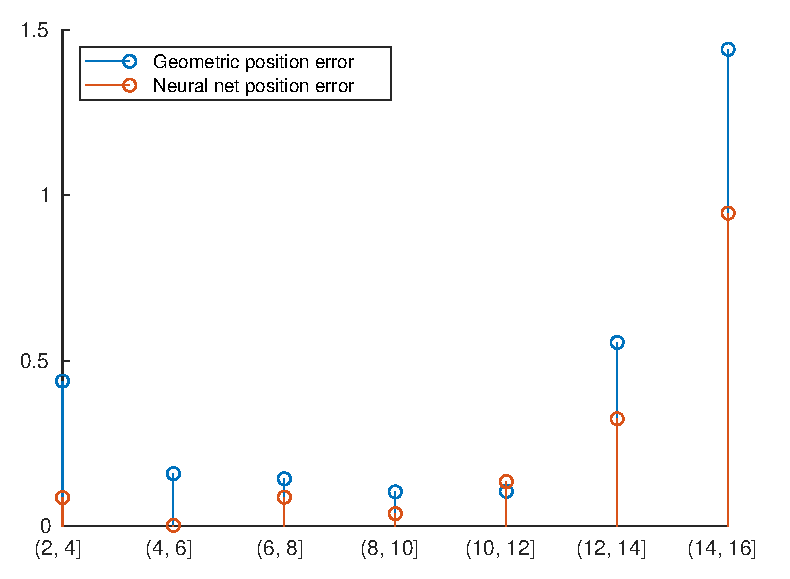
\includegraphics[width=0.8\linewidth]{0_Images/3_Theory/camDetection/rErrorCamera.eps}
    \caption[Error in the distance estimate of the two camera based detection approaches.]
    {Error in the distance estimate of the two camera based detection approaches.}
    \label{Fig:rErrorCamera}
\end{figure}

\begin{figure}
    \centering
    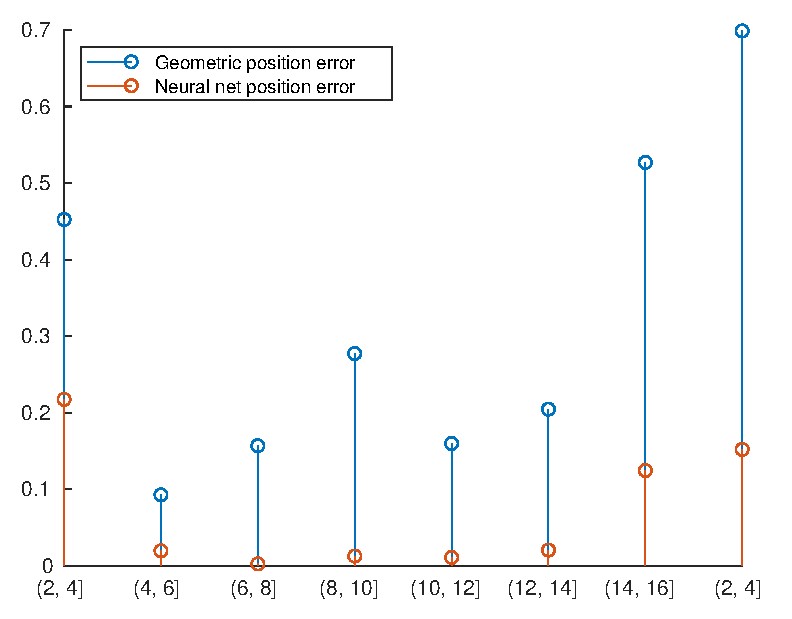
\includegraphics[width=0.8\linewidth]{0_Images/3_Theory/camDetection/psiErrorCamera.eps}
    \caption[Error in the angle estimate of the two camera based detection approaches.]
    {Error in the angle estimate of the two camera based detection approaches.}
    \label{Fig:psiErrorCamera}
\end{figure}

\fi